%%%%%%%%%%%%%%%%%%%%%%%%%%%%%%%%%%%%%%%%%%%%%%%%%%%%%%%%%%%%%%%%%%%%%%%%%%%%%%%%
\section{Scenario 3: Both Hosts on Wi-Fi, one Submerged in Seawater}

\label{sec:wifi_water}
\begin{figure}[h]
    \centering
    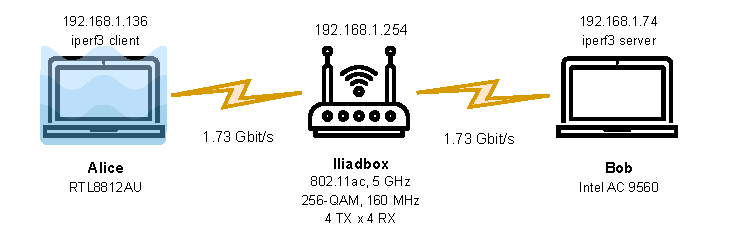
\includegraphics[width=0.95\linewidth]{images/wifi_water.drawio.pdf}
    \caption{Seawater scenario}
    \label{fig:wifi_to_wifi_water_pic}
\end{figure}

\subsection{Scenario description}
For our third test, we explore how Wi-Fi connections work underwater. This may happen in scenarios such as sensor analysis for water quality and oil spill detection, or submarine communications and mine detection and neutralization. We designed an experiment in which one Wi-Fi-connected host was submerged in seawater while the other host was not.
To replicate this, we enclosed the directional antenna in a waterproof silicone material. Subsequently, we submerged the antenna in 5 cm of water with a salt concentration of 35\%.

Our test setup consisted of the same two hosts with identical configurations in the previous scenario (\ref{sec:wifi}). The only variable introduced was the addition of water for the host equipped with the directional antenna.

\subsection{Consideration on the TMG}
The salinity of water significantly impacts electromagnetic (EM) wave propagation, leading to higher attenuation compared to free-space conditions. This is due to changes in the water's permittivity, which is influenced by the dipole moment of water molecules, and the increased conductivity resulting from the ionization of added salt. Pure water has low conductivity because its molecules are not naturally polarized, but the introduction of salt enhances conductivity, further increasing the EM wave attenuation.

Based on these factors, we expect a substantial reduction in throughput in saline water, primarily due to the high attenuation of EM waves. The increased conductivity and dielectric properties of seawater are likely to degrade signal quality and lower the data transfer rate. \cite{arrabitothesis}

In the previous experiment conducted in air, we observed a goodput of 192 Mbit/s under conventional conditions (\ref{sec:wifi}). However, when submerged in seawater, we anticipate that signal attenuation, potential multipath effects and wave absorption will significantly reduce goodput.


\subsection{Test results evaluation}


\begin{table}[H]
    \centering
    \caption{TCP Goodput from \texttt{iperf3} test (Mbps)}
    \label{tab:tcp-throughput-wifi}
    \begin{tabular}{lrrrrc}
        \hline
        \textbf{Reverse flag} & \textbf{Avg} & \textbf{Median} & \textbf{Min} & \textbf{Max} & \textbf{Std Dev} \\
        \hline
        False & 3.499 & 3.81 & 1.13 & 5.47 & 1.49 \\
        True & 9.914 & 9.985 & 5.86 & 14.6 & 2.72 \\
        \hline
    \end{tabular}
\end{table}
During the experiments we noted, observing the router's admin panel, how Alice's network card was hopping from one configuration to another. In particular, it autonomously downgraded its connection from the 5 GHz band to a slower standard in the 2.4 GHz band. In general, the results of this experiment align with our expectations regarding the impact of seawater on Wi-Fi performance. As discussed previously, the presence of saltwater significantly attenuates electromagnetic waves (EM), which in turn degrades the throughput and reliability of wireless networks. 

This scenario also reveals differences in signal performance between transmission and reception modes. Among the various reasons for this, we could consider the high unrealiability of the channel as the main cause. In fact, other technologies are often used for underwater communication. Acoustic waves, similar to sonar, are the most common method, as they travel efficiently through water and are used in submarines and underwater research (\ref{sec:underwater-comm}) \cite{arrabitothesis}.

Moving on to examine the sequence number graph for this scenario, we can immediately notice that the slope of the curve is less steep compared to previous scenarios. This suggests a lower overall throughput. 

\begin{figure}[H]
    \centering
    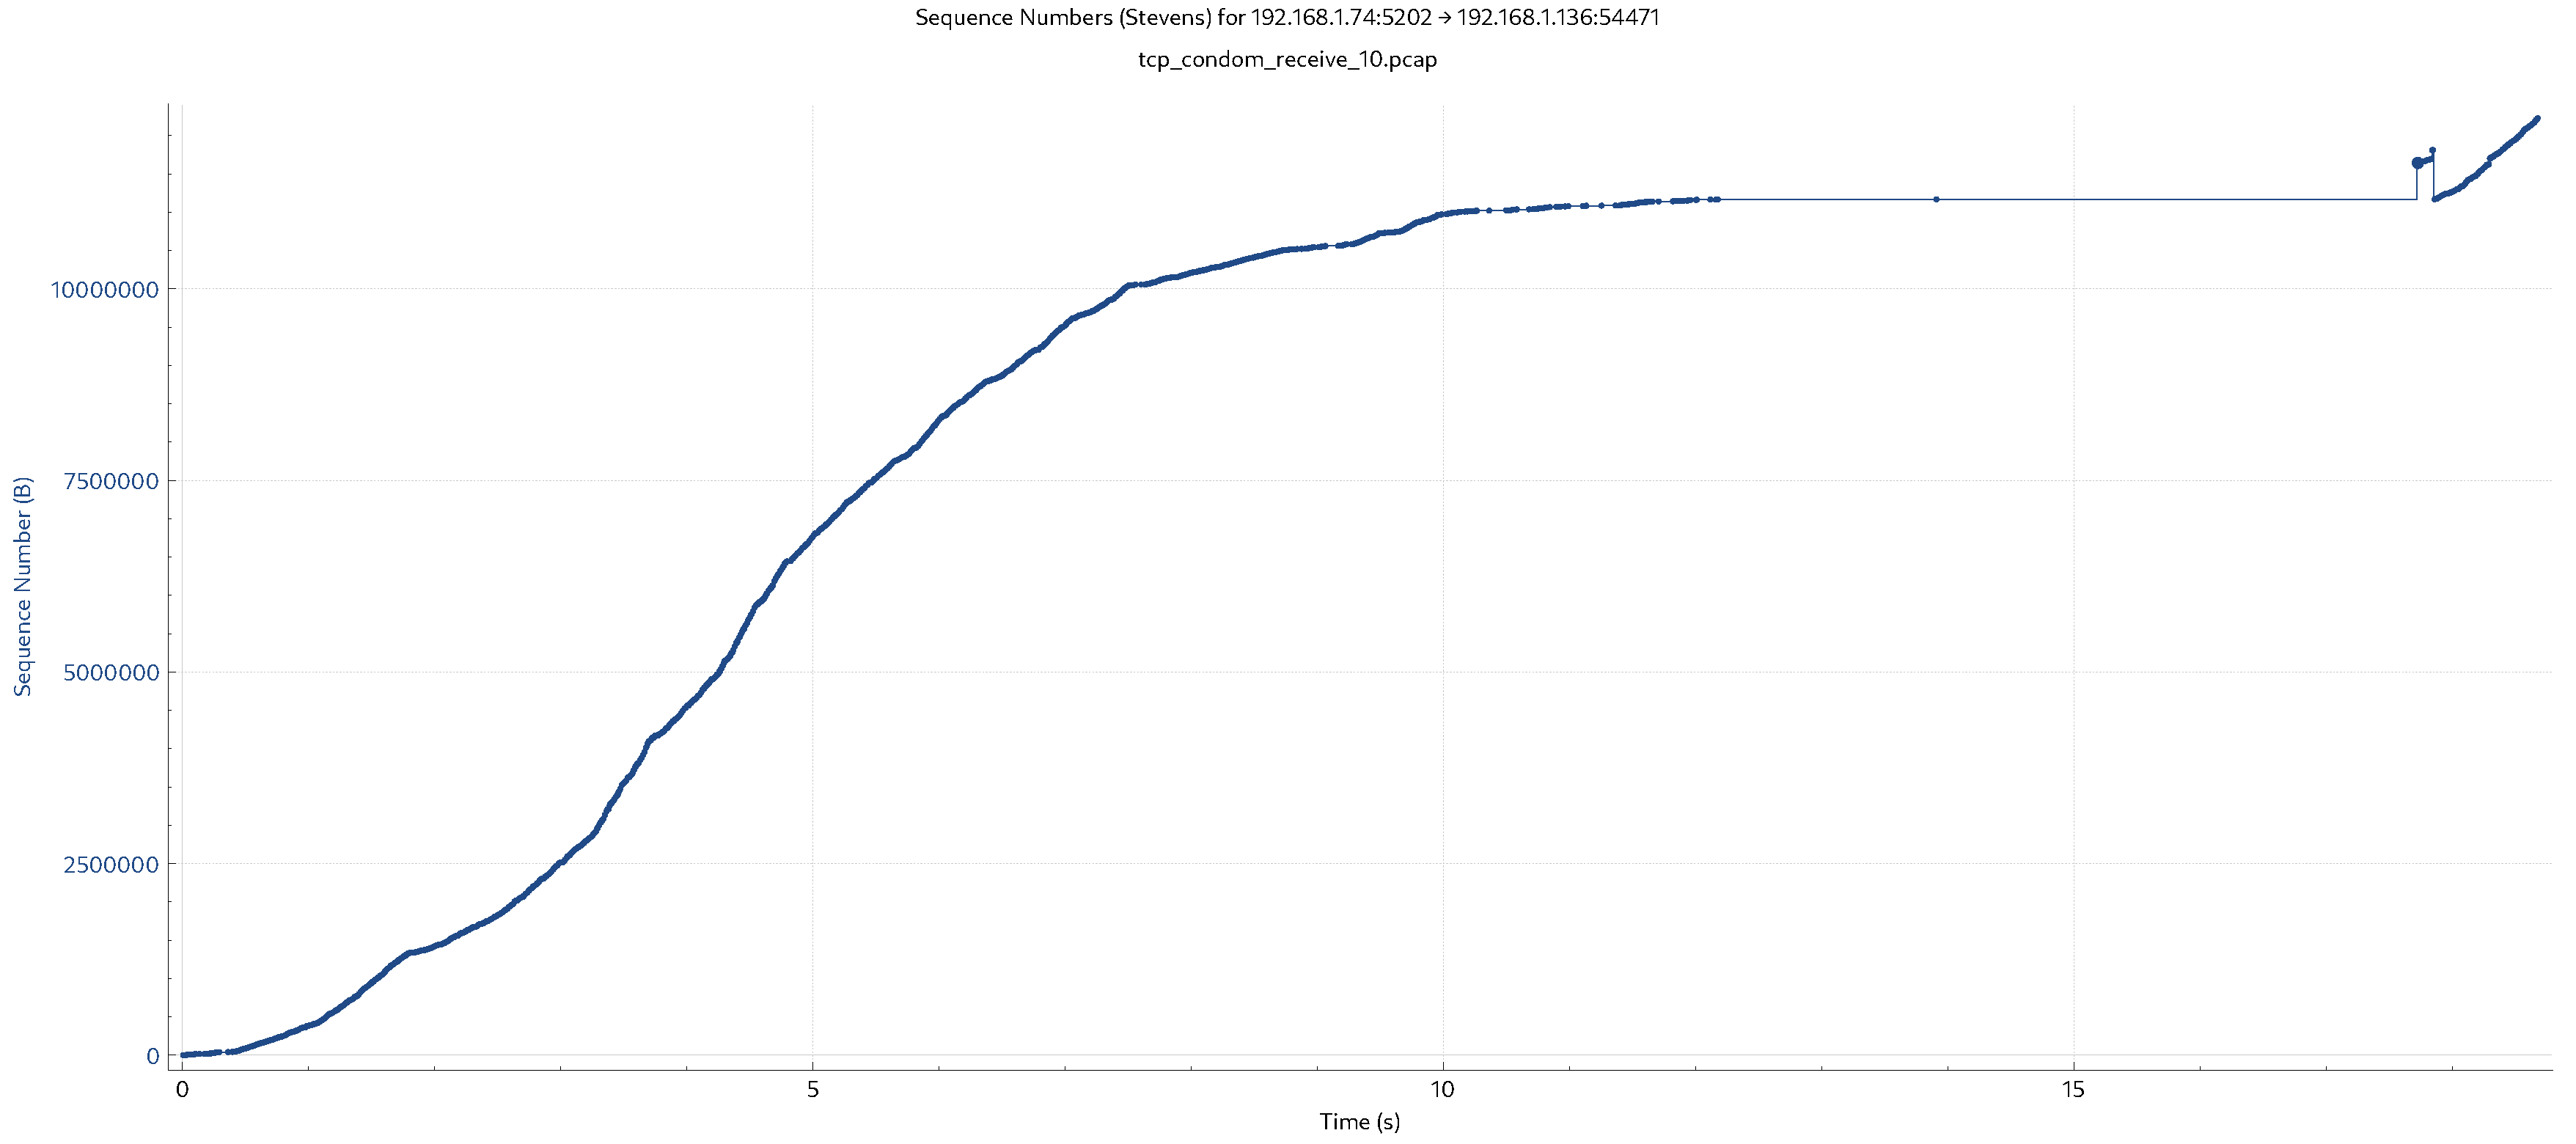
\includegraphics[width=0.75\linewidth]{images/SeqNumSaltWater.pdf}
    \caption{Sequence Numbers (Stevens), reverse flag set to True}
    \label{fig:enter-label}
\end{figure}

Additionally, the transmission lasted longer than the 10 seconds we set in the test parameters. 
This is evident from the graph, where towards the end of the transmission, the slope flattens (forming a horizontal line), indicating that no data was being received at that point. This is due to the need for retransmissions, as shown by the drop in the sequence number at one point. These retransmissions and the presence of duplicate ACKs are confirmed by using specific Wireshark filters and observing the TCP errors graph (\ref{graficoCiro}).

The second graph, which shows the outstanding bytes (bytes that have been sent but have not yet been acknowledged), further confirms that retransmissions occurred later in the transmission. This behavior can be better understood when examining the receiving window graph. The recWin shows how much data the receiver can accept at a given time. The recWin graph fluctuates continuously, suggesting that the system was adjusting dynamically due to network congestion or other factors. 

\begin{figure}[H]
    \centering
    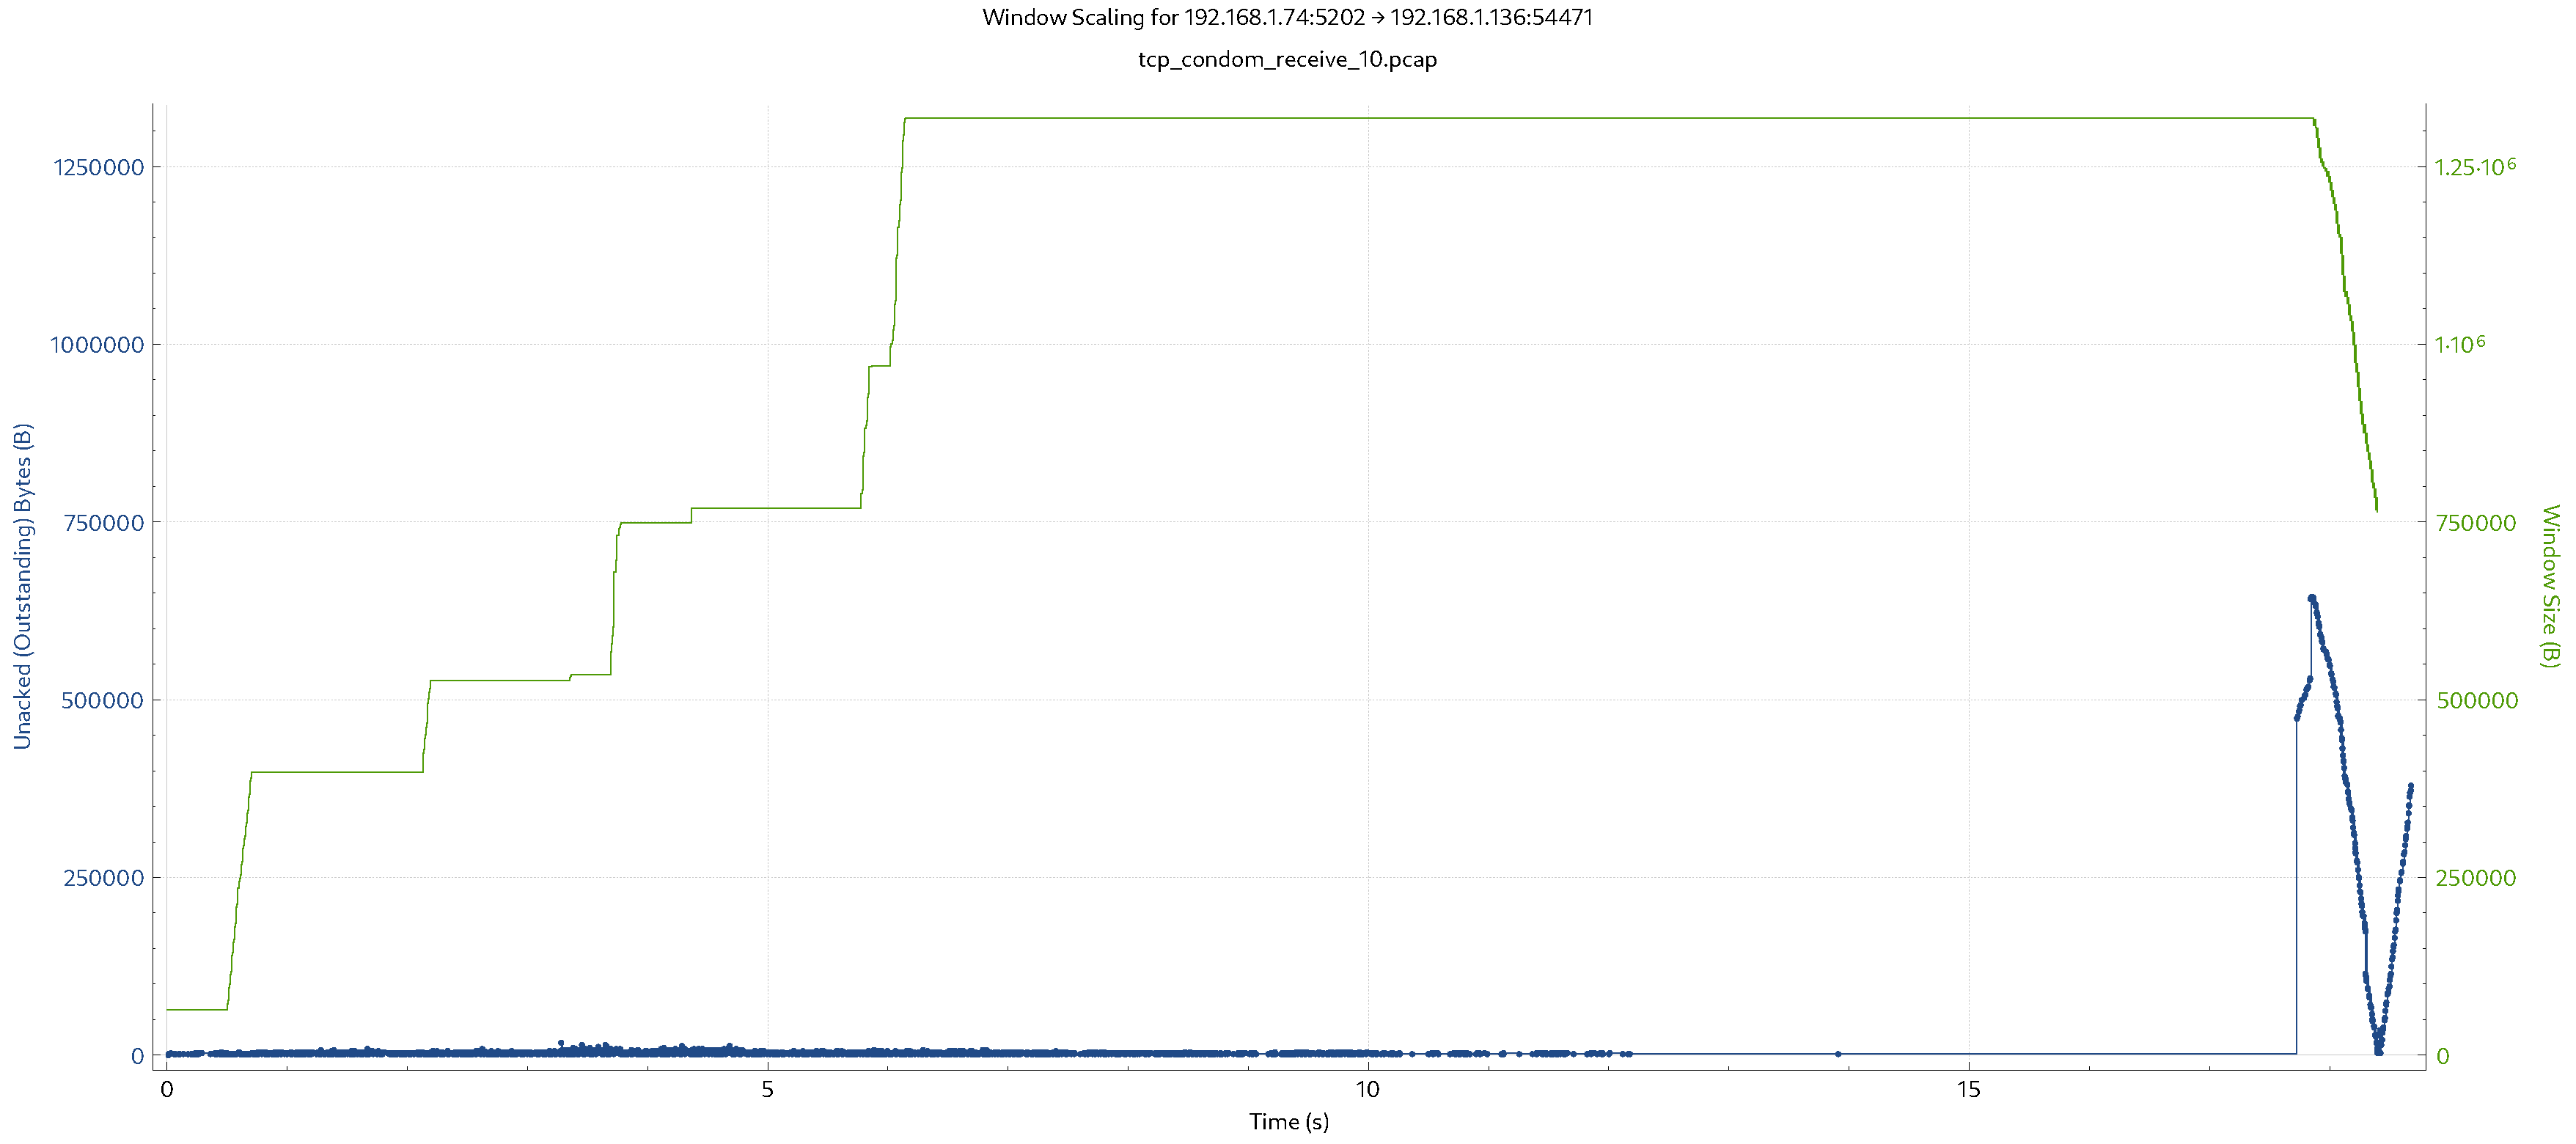
\includegraphics[width=0.75\linewidth]{RecWinSaltWater.pdf}
    \caption{OutBytes and recWin size on the client, reverse flag set to True}
    \label{fig:enter-label}
\end{figure}

Unlike other scenarios, where the recWin remains stable, the continuous change in this case indicates that the submerged receiver dynamically adjusted its window size, likely due to fluctuating network conditions during the test. This adjustment was a preventive measure to avoid overloading the receiver. In fact, if the receiver experiences high traffic or delays, it may reduce the window size to prevent overloading, causing fluctuations in the recWin even without the need for retransmission.

In conclusion, the experiment validated our initial predictions regarding the catastrophic impact of seawater on EM wave propagation.